% 依据固定源印刷页35；投影图不表示角度或比例。
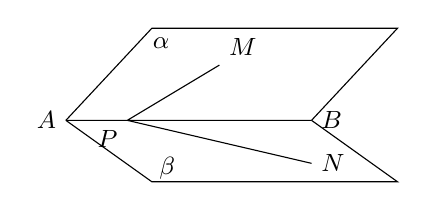
\begin{tikzpicture}[scale=0.78,font=\small]
  \coordinate (A) at (0,0);
  \coordinate (B) at (4,0);
  \coordinate (P) at (1,0);
  \coordinate (M) at (2.5,0.9);
  \coordinate (N) at (4,-0.7);
  \draw (A)--(1.4,1.5)--(5.4,1.5)--(B);
  \draw (A)--(1.4,-1)--(5.4,-1)--(B);
  \draw (A)--(B) (P)--(M) (P)--(N);
  \node[left] at (A) {$A$};
  \node[right] at (B) {$B$};
  \node[below left] at (P) {$P$};
  \node[above right] at (M) {$M$};
  \node[right] at (N) {$N$};
  \node at (1.55,1.25) {$\alpha$};
  \node at (1.65,-0.78) {$\beta$};
\end{tikzpicture}
